\chapter{Introducción}

\minitoc
	
\section{Introducción}

Este documento contiene la memoria del Trabajo Fin de Grado realizado por Ignacio Agüero Salcines para la obtención del título de Grado en Ingeniería Informática. Dicho trabajo Trabajo Fin de Grado fue realizado en la empresa CIC Consulting Informático, entre los meses de XXX y XXX de 2017 y 2018. Durante ese periodo el alumno realizó una carga total de trabajo de XXX, bajo la supervisión de XXX dentro del Departemento de XXX.

El presente trabajo se enmarca concretamente dentro del proyecto LUCA. El objetivo general de dicho proyecto es proporcionar una interfaz de acceso uniforme a un conjunto de fuentes de datos heterogéneas. El proyecto LUCA, el cual se describirá en mayor profundidad en la siguiente sección, comenzó en XXX, está actualmente en fase de XXX, (si está en producción, indicar a cuántos clientes se ha vendido) e involucra a XXX trabajadores.

El proyecto descrito en este trabajo se enmarca dentro del proyecto LUCA y tiene como objetivo facilitar los procesos de recuperación de información que requieren de la realización de consultas encadenadas donde las salidas de unas consultas se utilizan como entradas para otras. A este conjunto de consultas encadenadas los denominaremos en adelante \emph{procesos}. 

Dado que para entender los objetivos de este proyecto es necesario antes conocer cuáles son los objetivos de LUCA y cómo funciona dicha herramienta, la siguiente sección proporciona una breve introducción a la herramienta LUCA.

\section{LUCA}

\subsection{Motivación}

En los últimos años, el volumen de datos recogidos y manipulados por las empresas ha aumentado de forma vertiginosa. Estos datos se han ido almacenando en diferentes tipos de fuentes conforme las empresas crecían y sus sistemas evolucionaban y se fusionaban. Como resultado de  este proceso no es extraño actualmente encontrar empresas que tengan sus datos almacenados en sistemas tan dispares como bases de datos relacionales, hojas XML o repositorios FTP.

Como consecuencia de esta nueva situación, cuando un usuario quiere obtener una información concreta cuyos datos residen en varios de estos sistemas, éste necesita acceder a cada uno de estos sistemas, extraer de cada sistema la información que precisa, y finalmente filtrarla y unificarla para finalmente obtener los datos requeridos.

Por ejemplo, una cadena de venta de electrodomésticos podría tener sistemas informáticos diferentes para el departamento de atención al cliente, para el departamento técnico de postventa y para el departamento de compras y adquisiciones. Por tanto, para conocer con precisión el estado actual de una reparación, podríamos necesitar:

\begin{enumerate}
	\item Acceder al sistema de atención al cliente para obtener el identificador de la incidencia y en qué fase de su gestión se encuentra.
	\item Una vez corroborado que la incidencia está actualmente siendo atendida, recuperaríamos del sistema de gestión de reparaciones el estado detallado de la reparación. Como resultado de esta operación, supongamos que averiguamos que la reparación está a la espera de recibir una pieza que se ha de sustituir.
	\item Finalmente, para poder hacer una estimación de cuando podría estar lista la reparación, accederíamos al sistema de compra y adquisiciones para averiguar cuando está prevista la entrega de la pieza solicitada.
\end{enumerate}

Como hemos comentado anteriormente, a cada uno de estos sistemas podría accederse de manera diferente. Por ejemplo, el primero podría consultarse utilizando un servicio web. La información del segundo podría recuperarse accediendo directamente a una base de datos relacional, mientras que la información del tercero se obtendría analizando órdenes de compra en formato \emph{pdf} almacenadas en un repositorio de ficheros compartido. Por tanto, el usuario, para poder realizar este proceso, necesita conocer las particularidades de cada sistema y de su forma de acceso.

Para aliviar esta situación, dentro de la empresa CIC, se está desarrollando una aplicación denominada LUCA, a la cual contribuye este Trabajo Fin de Grado. Para facilitar este proceso de recuperación de información, LUCA proporciona un lenguaje común para todas las fuentes de datos a unificar, permitiendo al usuario abstraerse de los detalles de cada fuente.

\subsection{Funcionamiento de LUCA}

A continuación, se detalla brevemente el funcionamiento de \emph{LUCA}. Para ello, utilizaremos como ejemplo una consulta a la base de datos de LUCA, esta consulta obtendrá los procesos en función de un estado (los estados pueden ser en edición, publicado, es decir, preparada para ser ejecutada, o borrado).

\begin{figure}[!tb]
    \centering
 	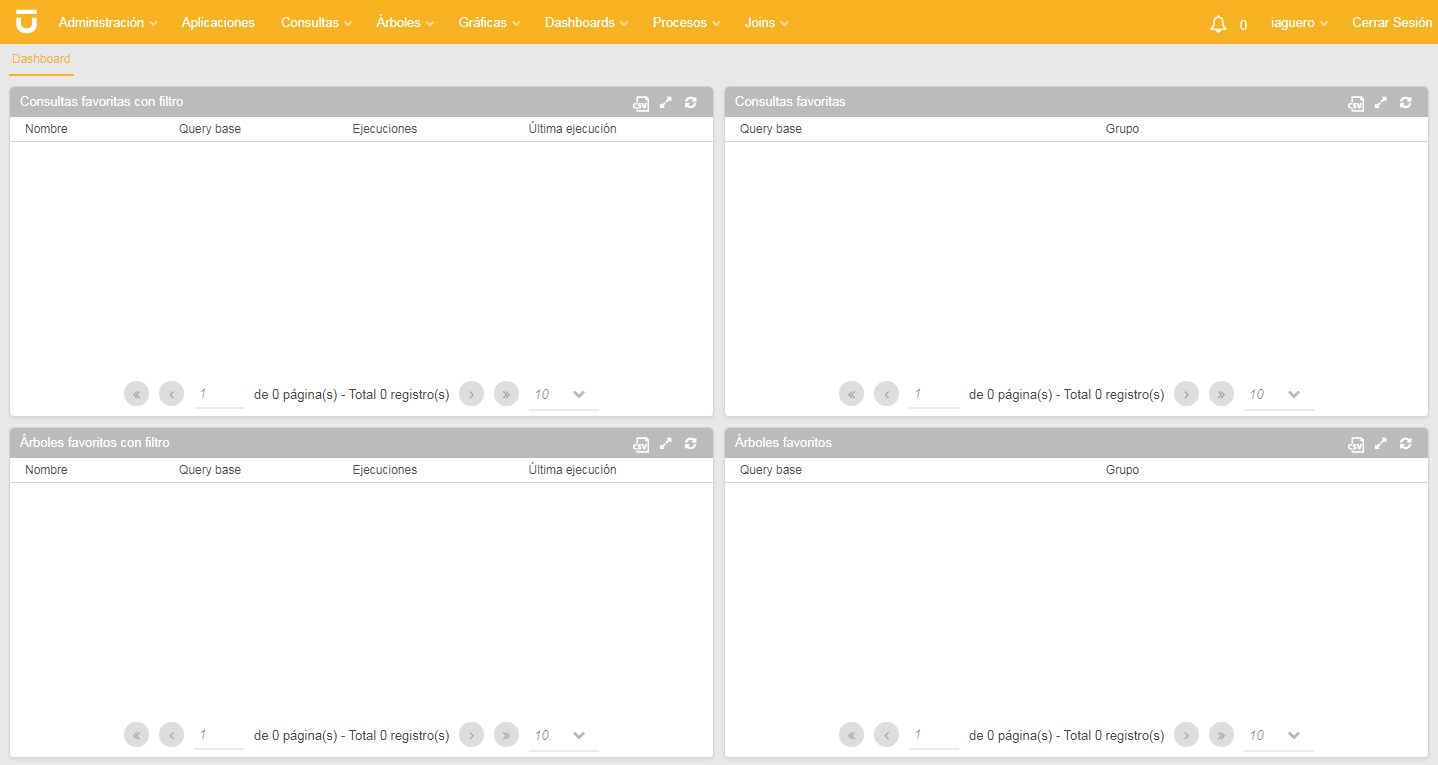
\includegraphics[width=\linewidth]{capturasLuca/menuLuca.png}
	\caption{Menu Principal LUCA}
    \label{fig:menuLuca}
\end{figure}

En el menu principal de LUCA, nos aparece una vista con un conjunto de consultas que el usuario ha marcado como favoritas (Figura~\ref{fig:menuLuca}), es decir, que suele utilizar con frecuencia. Como se dijo anteriormente, se utilizará la consulta de los procesos por estado.

\begin{figure}[!tb]
	\centering
	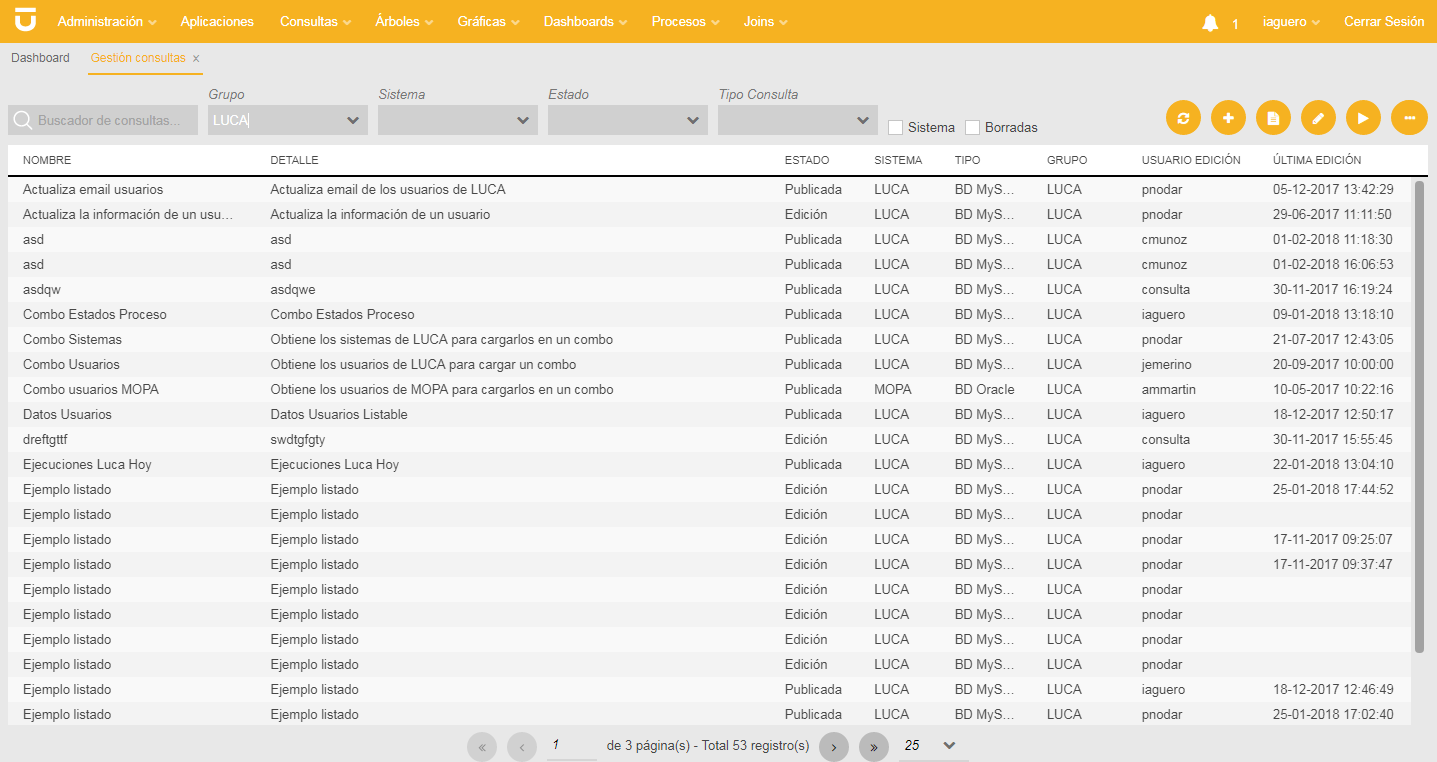
\includegraphics[width=\linewidth]{capturasLuca/gestionConsultas.png}
	\caption{Vista de Gestión de Consultas}
	\label{fig:gestionConsultas}
\end{figure}

En la vista de gestión de consultas (Figura~\ref{fig:gestionConsultas}) se pueden realizar las operaciones propias de la gestión, como es crear, modificar, eliminar o ejecutar entre otras.

No obstante, para que dichas consultas pueden ser ejecutadas, es necesario un usuario con conocimientos suficientes para ello, al que denominaremos en adelante el \emph{creador de consultas}.

\begin{figure}[!tb]
	\centering
	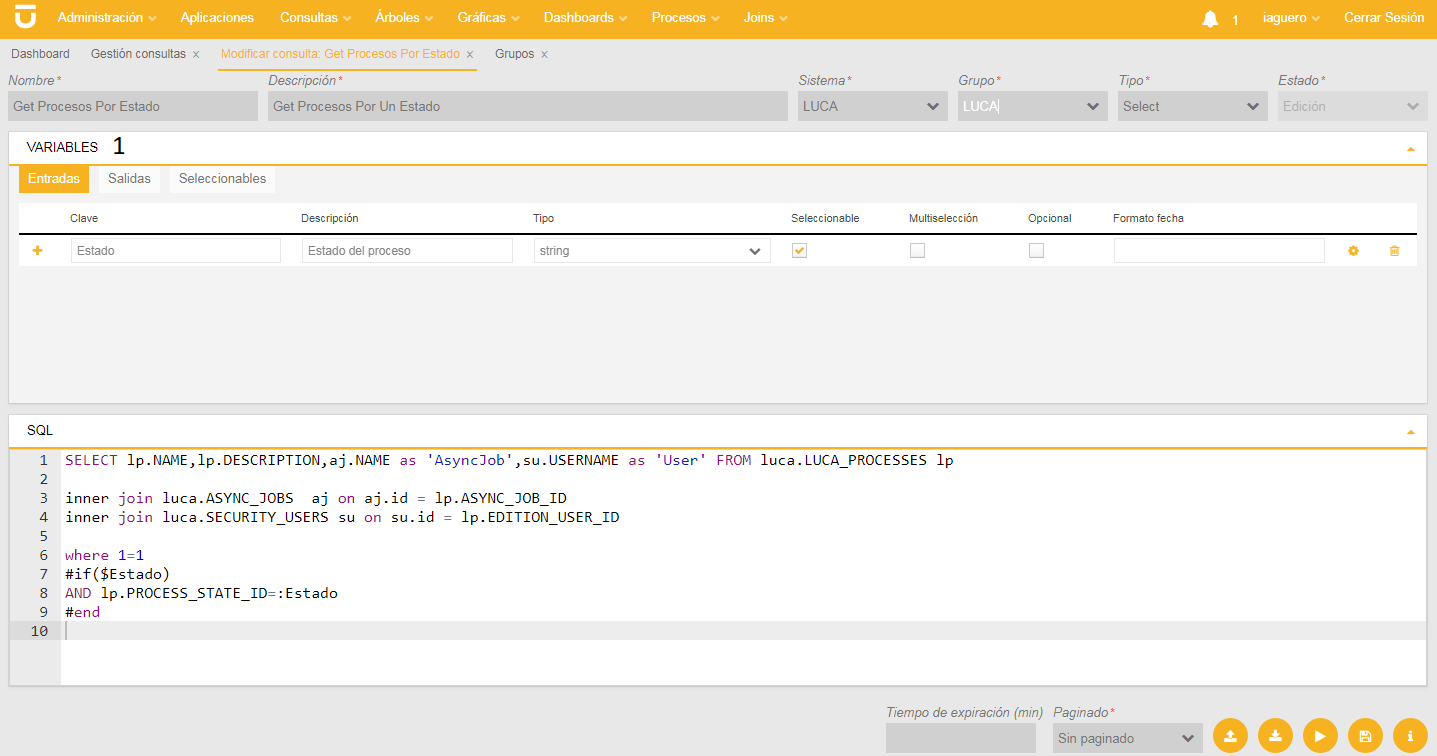
\includegraphics[width=\linewidth]{capturasLuca/creacionConsulta.png}
	\caption{Creación de una Consulta}
	\label{fig:creacionConsulta}
\end{figure}

Para poder realizar esta tarea, el creador de consultas accedería a la interfaz dedicada a esta tarea (ver Figura~\ref{fig:creacionConsulta}). En esta interfaz, definiría primero las variables de entrada y salida de la consulta (Figura~\ref{fig:creacionConsulta}, etiqueta 1). A continuación, especificaría cómo llevar a cabo dicha consulta a bajo nivel. Para ello puede utilizar una serie de facilidades y primitivas proporcionadas por LUCA. Para la consulta ejemplo, utilizando estas facilidades, se especifica que se desea obtener el nombre, la descripción, el nombre de la tarea asíncrona y el usuario, y se establece como variable de entrada el estado del proceso.

Tras guardar la consulta se puede ejecutar directamente desde la ventana de creación, sin embargo, si la consulta ya ha sido ejecutada previamente y el usuario la ha publicado (tras ejecutar una consulta desde la ventana de creación, si se ha ejecutado correctamente se le permite al usuario cambiar su estado de edición a publicada, esto significa que la consulta está preparada para ser ejecutada), el usuario puede ir a la ventada de ejecución de consultas, y desde ahí ejecutarla.

La principal ventaja que aporta LUCA es que el proceso de ejecución de consultas es opaco para el usuario que la ejecuta. El usuario sólo tiene que proporcionar los parámetros necesarios de entrada y seleccionar un formato de salida. Por tanto, el proceso de ejecución de consultas es exactamente el mismo con independencia de la fuente a la cual se accede.

Por ejemplo, en el caso de la consulta \emph{Get Procesos Por Estado} sería necesario proporcionar el estado de los procesos de los que queremos obtener información. Una vez introducido dicho estado, se seleccionaría el botón de ejecución de la consulta (Figura~\ref{fig:ejecucionConsulta}, etiqueta 2). Finalmente, se muestra el resultado de la consulta, el cuál puede ser visualizado de diferentes formas en función del recurso al que se llama. En nuestro caso, se muestra como una tabla ya que es una consulta a base de datos (Figura~\ref{fig:ejecucionConsulta}, etiqueta 3).

Lo importante de este proceso es que, una vez definida la consulta, ésta se puede ejecutar fácilmente sin conocer los detalles internos de la misma, incluso hasta el tipo de sistema al que se accede.

	\begin{figure}[!tb]
		\centering
		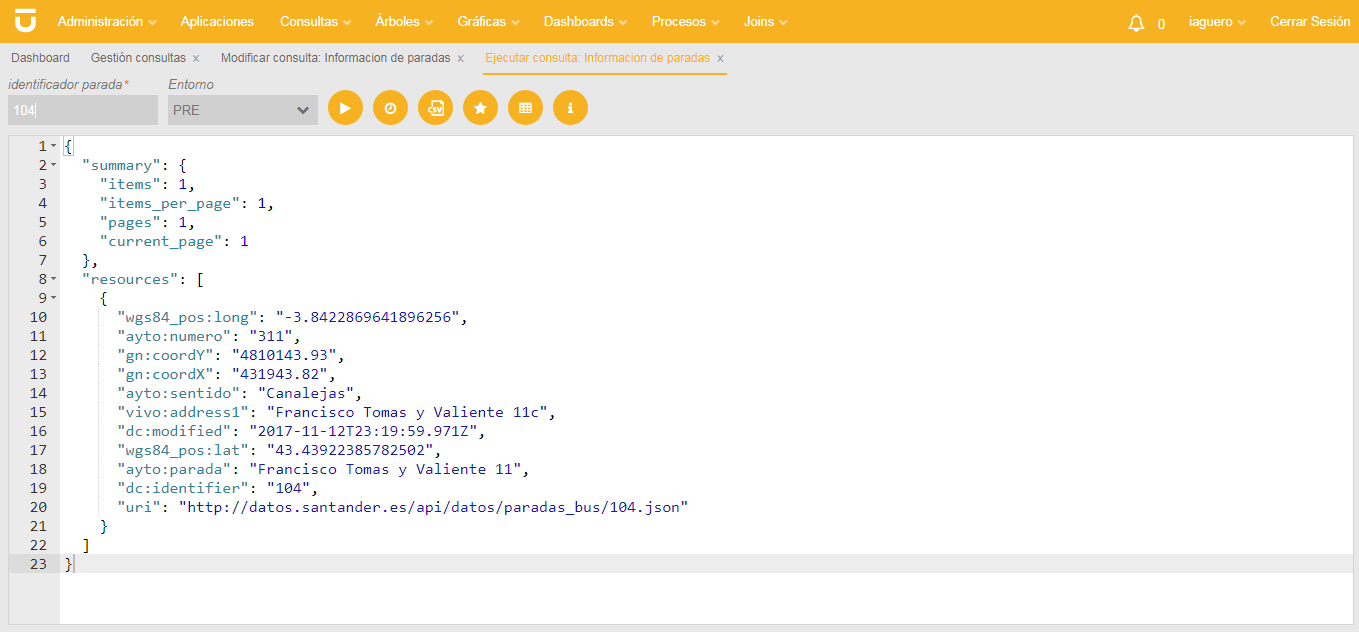
\includegraphics[width=\linewidth]{capturasLuca/ejecucionConsulta.png}
		\caption{Vista de Ejecución de Consultas}\label{fig:ejecucionConsultas}
	\end{figure}

\subsection{Limitaciones actuales de LUCA}

Actualmente, LUCA proporciona mecanismos para permitir al usuario recuperar de manera uniforme información de diferentes fuentes de datos. No obstante, LUCA por el momento sólo es capaz recuperar información de una única fuente de datos a la vez. Por tanto, cuando es necesario combinar información procedente de distintas fuentes, el propio usuario es el que debe realizar dicho proceso de composición a mano, ejecutando él cada consulta, y utilizando las salidas de cada una de ellas como entradas para las siguientes.


Un ejemplo de dicho proceso de composición sería la necesidad de un dependiente de una tienda de electrodomésticos de obtener la edad de los usuarios que compraron lavadoras durante el mes pasado. Actualmente, la secuencia de consultas que debería de realizar serían las siguientes:

\begin{itemize}
	\item Primero necesitaría obtener el registro de compras del mes pasado del sistema.
	\item Después, tras guardar dicho registro, tendría que, uno por uno, seleccionar los que se corresponden con lavadoras.
	\item Una vez que el usuario tiene las lavadoras compradas el mes pasado, éste tendría que extraer que usuarios han comprado las lavadoras.
	\item Por último, debería buscar en el sistema cada usuario que ha realizado la compra, a partir del nombre obtenido en el punto anterior, y anotar su edad.
\end{itemize}

En adelante, estas cadenas de consultas para obtener un resultado concreto las denominaremos \emph{procesos}. El problema actual de LUCA, tal como ilustra el ejemplo anterior, es que no soporta el concepto de \emph{proceso}. Por tanto, para ejecutar un proceso,  el usuario tiene que realizar una larga y compleja secuencia de acciones.

\section{Objetivos del Trabajo de Fin de Grado}

El objetivo general de este Trabajo Fin de Grado es integrar en LUCA el concepto de \emph{proceso}. Para ello, hay que dar soporte a dos cuestiones diferentes: (1) la ejecución de los procesos; y (2) la especificación de procesos. Por tanto, el objetivo general de este trabajo se descompone en estos dos subobjetivos principales.

El primer objetivo implica poder tratar procesos en LUCA de la misma forma que se trata las consultas. Es decir, los procesos deberán aparecer como en las consultas bajo una pestaña de gestión y otra de ejecución. Obviamente, la complejidad de ejecutar una proceso es mayor que la de ejecutar una consulta, ya que necesitamos ejecutar varias consultas, guardar resultados intermedios y utilizar estos resultados como entradas para otras consultas.

El segundo objetivo, que es el que implica una mayor complejidad, consiste en facilitar la especificación de procesos en LUCA. Para que un proceso pueda ser ejecutado, primero debe ser especificado, indicando qué consultas lo componen y cómo se relacionan. De acuerdo con los deseos expresados por los responsables del proyecto LUCA y la empresa CIC, dicho mecanismo de especificación debía ser gráfico, permitiendo así componer consultas de manera visual mediante la interconexión de las salidas de unas con las entradas de otras.

\section{Alcance del Proyecto}

Para refinar estos dos grandes objetivos en una serie de requisitos más concretos, se llevó a cabo en primer lugar una reunión con el Jefe y el Gerente del proyecto. El objetivo de dicha reunión era conocer LUCA en profundidad. A continuación, se nos proporcionaron unos documentos técnicos con los requisitos técnicos tanto para la ejecución de procesos como para el desarrollo del componente gráfico de especificación de procesos. Estos documentos pueden encontrarse en el Anexo adjunto a la memoria. Por tanto, dado que la fase de Ingeniería de Requisitos para este proyecto ya había sido realizada por la propia empresa, no era necesario repetirla dentro de este proyecto. 

Por otro lado, el proyecto a desarrollar debía integrarse dentro del proyecto LUCA, el cual ya tenía una arquitectura perfectamente definida. Por tanto, el presente proyecto simplemente debía seguir dichas pautas arquitetónicas, no siendo necesario tampoco realizar una fase de diseño arquitectónico del mismo. 

Consecuentemente, el proyecto queda reducido a las fases de diseño microarquitectónico pruebas y despliegue, aunque como es lógico, ésta última fase sería responsabilidad última de la dirección técnica del proyecto LUCA, al ser éstos los encargados de mantener la integridad del producto.

Estas fases de diseño y prueba se realizaron mediante un esquema de desarrollo iterativo e incremental, similar a de las metodologías ágiles, pero sin llegar a adoptar una elementos propios de un proyecto ágil, tales como un \emph{Product Backlog} o la limitación de la duración de las iteraciones a un tiempo concreto.

El desarrollo del producto se dividió en varias iteraciones. En cada iteración, se añadían nuevas funcionalidades al producto, que iba creciendo en complejidad. Al final de cada iteración, se mostraba el producto a los responsables del proyecto LUCA, los cuales daban su aprobación para continuar con el desarrollo y sugerían los cambios y modificaciones que consideraban oportunos. 

%%==============================================================================%%
%% NOTE(Pablo): Lo de abajo se quita por simplicidad                            %%
%%==============================================================================%%
%%
%% Como ya se ha mencionado, en estos documentos se pueden encontrar los
%% requisitos técnicos atribuidos al proyecto, pero, de forma resumida, se
%% centran en tres pilares o requisitos principales:
%%
%% \begin{itemize}
%%  	\item Concatenación de las consultas entre si pertenecientes a un
%%            mismo proceso.
%% 	\item Visualización del progreso de ejecución del proceso.
%% 	\item Aplicar criterios de navegación a partir de los resultados de salidas.
%% \end{itemize}
%%
%%
%%==============================================================================%%
%%
%% Comentar que la arquitectura ya estaba definida, por lo que el proyecto se reduce
%% a las fases de diseño detallado, implementación y pruebas.
%%
%% El proyecto genera como resultado dos módulos grande y bien diferenciados:
%%    Process Editor Component y (se va a cambiar).
%%==============================================================================%%

\section{Sumario}

Este capítulo ha presentado los objetivos del proyecto descrito en este documento. El objetivo general de dicho proyecto era permitir que la herramienta LUCA soportase el concepto de \emph{proceso}, entendiéndose por \emph{proceso} la ejecución de una serie de consultas concatenadas de recuperación de la información donde las salidas de ciertas consultas sirven como entradas para otras. 

Antes de entrar a profundizar y refinar dicho objetivo, se ha descrito la herramienta LUCA, detallando sus objetivos generales, su estado actual y sus limitaciones. Seguidamente, se han introducido los objetivos concretos de este proyecto, consistentes en aliviar parte de las limitaciones actuales de LUCA. Finalmente se ha definido el alcance concreto del proyecto, resaltando que las fases de Ingeniería de Requisitos y Diseño Arquitectónico quedan fuera del mismo.